
\documentclass{article}
\usepackage{graphicx}
\setlength{\parindent}{0pt}
\setlength{\parskip}{\baselineskip}
\usepackage{listings}

\newenvironment{qanda}{\setlength{\parindent}{0pt}}{\bigskip}
\newcommand{\Q}{\bigskip\bfseries Q: }
\newcommand{\A}{\par\textbf{A:} \normalfont}


\begin{document}

\title{Development of Real-Time Systems: Assignment 2}
\author{Ross Owen}
\maketitle

\section{Unblock Comms Without Modifying Tasks}
The "communicationtask" must send a simulated data packet every 200ms but is often blocked by "matrixtask". In order to fix this problem without modifying the task the priority of the tasks must be modified.

In FreeRTOS each task is assigned a priority from 0 to configMAX\_PRIORITIES - 1, where configMAX\_PRIORITIES is defined within FreeRTOSConfig.h.
Initially the communications task is set to priority 3 and matrix task set to priority 1 and therefore the Matrix task has been set to a higher priority than the Communications task.

Reversing the priority of these two tasks resolves the issue without modifying the either of the code in the two tasks.

\subsection{Proof \& Testing}

In order to prove this was the case a quick test was authored to measure how often the Communications was was being called.
This was based on \verb|xTaskGetTickCount()| which returns the count of ticks since \verb|vTaskStartScheduler()| was called.

\begin{lstlisting}[language=C]
static void communication_task()
{
    TickType_t prevTickCount = xTaskGetTickCount();
    TickType_t curTickCount;
    
    while (1) 
    {
        /* Measurement */
        curTickCount = xTaskGetTickCount();
        TickType_t tickDiff = curTickCount - prevTickCount;
        prevTickCount = curTickCount;
        printf("TickCount: %d\n", tickDiff);    

        /* Original task code */
        printf("Sending data...\n");
        fflush(stdout);
        vTaskDelay(100);
        printf("Data sent!\n");
        fflush(stdout);
        vTaskDelay(100);
    }
}
\end{lstlisting}

With the original priorities the output (as shown below) shows that the communications task is blocked for longer the 200ms.

\begin{lstlisting}
TickCount: 897
Sending data...
Data sent!
TickCount: 900
Sending data...
Data sent!
TickCount: 905
Sending data...
Data sent!
TickCount: 890
Sending data...
Data sent!
TickCount: 897
Sending data...
Data sent!
TickCount: 891
Sending data...
Data sent!
TickCount: 893
Sending data...
Data sent!
\end{lstlisting}

By increasing the priority of communications task to a priority higher than matrix task (say 2 and 1 respectively) the output belows shows that the
communications task can run every 200ms as required:

\begin{lstlisting}
TickCount: 200
Sending data...
Data sent!
TickCount: 200
Sending data...
Data sent!
TickCount: 200
Sending data...
Data sent!
TickCount: 200
Sending data...
Data sent!
TickCount: 200
Sending data...
Data sent!
TickCount: 200
Sending data...
Data sent!
\end{lstlisting}


\section{Adding ``prioritysettask''}

Since the assignment hints at the use of \verb|vApplicationTickHook()| the timing methodology was change to a simple global being incremented in this hook:

\begin{lstlisting}
void vApplicationTickHook( void )
{
    g_tickCount++;
}
\end{lstlisting}

"matrixtask" and "communicationtask" use this global counter to time their period/execution time.

A task "prioritysettask" was added to modify the priority of "communicationtask" based on it's execution time. This was achieved using \verb|vTaskPrioritySet()| and the handle of the task.


\section{Questions}

\begin{qanda}

\Q Why is "matrixtask" using most of the CPU utilization?

\A ``matrixtask'' is performing matrix multiplications on a 10x10 matrix, this is a computationally expensive operation due to the number of arithmetic operations (N multiplications and N additions for one result element, N\textsuperscript{3} multiplications and additions for all result elements) and memory accesses required.  This is exasperated if emulating floating point arithmetic an embedded platform without a floating point unit - this is simulated by the ``simulation'' delay loop. 


\Q Why must the priority of "communicationtask" increase in order for it to work properly

\A When the priority of "communicationtask" is less than "matrixtask" it only has the opportunity to be issued when "matrixtask" runs \verb|vTaskDelay()| and is blocked. By increasing its priority it can preempt the "matrixtask" allowing it to hit it's deadline.  

\Q What happens to the completion time of "matrixtask" when the priority of "communicationtask" is increased?

\A The completion time of "matrixtask" increased when the priority of "communcationtask" is increased. This is due to "matrixtask" being preempted by "communicationtask" to perform its required periodic communication. It can see by the trace that "matrixtask" timing jumps from 2.3ms to around 2.5ms as the priority of "communicationstask" increases.

\Q How many seconds is the period of "matrixtask"?

\A The period of "matrixtask" is approximately 2.3ms (optimisations turned off) in my environment.

\end{qanda}


\section{Final Output}

The final program output shows "matrixtask" blocking "communicationtask", the priorities are then updated such that "communcationtask" hits it's 200ms target, with "matrixtask" continuing to run:

\begin{figure}
    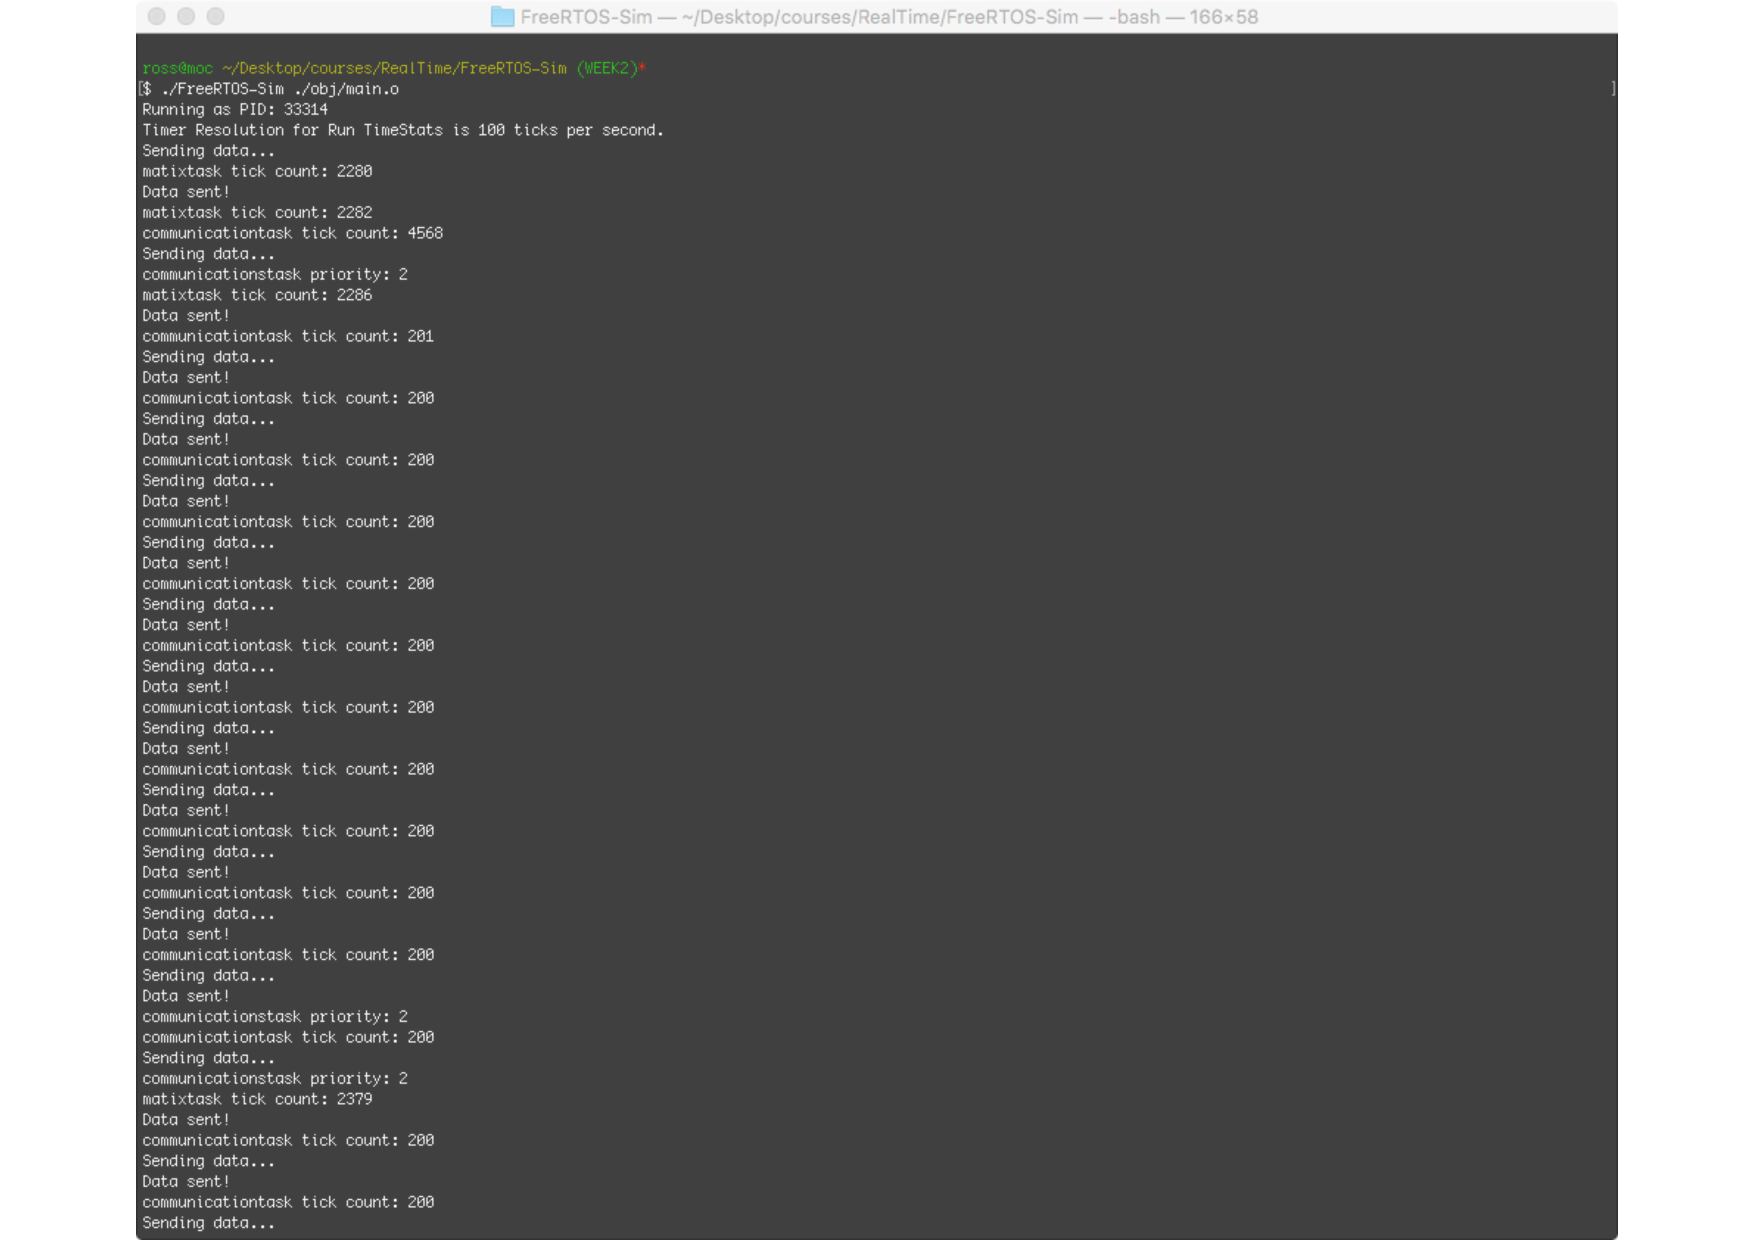
\includegraphics[width=10.0in]{week2}
    \caption{Simulation Results}
    \label{simulationfigure}
\end{figure}


\end{document}

